\part{Systems-of-DEs}
\lecture{Systems of DEs}{Systems-of-DEs}
\section{Systems of DEs}


\title{Ordinary Differential Equations}
\subtitle{Math 232 - Solving Systems of Differential Equations}
\date{31 October 2012}

\begin{frame}
  \titlepage
\end{frame}

\begin{frame}
  \frametitle{Outline}
  \tableofcontents[pausesection,hideothersubsections]
\end{frame}


\subsection{Systems of Differential Equations}


\begin{frame}
  \frametitle{Systems of Differential Equations}

  Conceptual Model: Coupled System \\
  \centerline{\includegraphics[width=7cm]{img/doubleSpringMass}}

  \begin{eqnarray*}
    \deriv{~}{t} \lp m \vec{v_1} \rp & = & \sum_j \vec{F}_{1j} \\
    \deriv{~}{t} \lp m \vec{v_2} \rp & = & \sum_j \vec{F}_{2j} 
  \end{eqnarray*}

  \uncover<2->{%
    These two equations depend on each other.
    }

\end{frame}


\begin{frame}
  \frametitle{Vicini - He Told Me to Go Back To The Beginning}

  \begin{eqnarray*}
    \deriv{~}{t} x_1  & = & a_{11} x_1 + a_{12} x_2 + f_1(t), \\
    \deriv{~}{t} x_2  & = & a_{21} x_1 + a_{22} x_2 + f_2(t).
  \end{eqnarray*}

  Writing the system in matrix/vector form we get
  \begin{eqnarray*}
    \deriv{~}{t} \vecTwo{x_1}{x_2} & = & 
    \arrayTwo{a_{11}}{a_{12}}{a_{21}}{a_{22}} \vecTwo{x_1}{x_2} + 
    \vecTwo{f_1}{f_2}.
  \end{eqnarray*}

\end{frame}


\begin{frame}
  \frametitle{More General Notation}

  \begin{eqnarray*}
    \deriv{~}{t} \vec{x}(t) & = & A(t) \vec{x}(t) + \vec{f}(t), \\
    \deriv{~}{t} \vec{x} & = & A \vec{x} + \vec{f}, \\
    \vec{x}(t_0) & = & \vec{c} 
  \end{eqnarray*}

  If $\vec{f}=\vec{0}$ then the system of equations is
  {\color{red}homogeneous}. 
  Otherwise, the system is {\color{red}nonhomogeneous}.

  {\color{blue}Remark:} 
  \begin{itemize}
  \item Solutions are the sum of homogeneous and particular solutions.
  \item Solutions are found by assuming a general form and then
    searching for the ``right answer.''
  \end{itemize}

\end{frame}

\subsection{Example}

\iftoggle{clicker}{%
\begin{frame}
  \frametitle{Clicker Quiz}

   \ifnum\value{clickerQuiz}=1{%

    \vfill
   \begin{eqnarray*}
     \deriv{~}{t} x_1 & = & 5  x_1 + 24 x_2 + 8 e^{-11t}, \\
     \deriv{~}{t} x_2 & = & -2 x_1 -  9 x_2 + 4 e^{-11t}.
   \end{eqnarray*}

   Written in matrix/vector form we get\\[12pt]

   \begin{tabular}{ll}
          A: &  $\deriv{~}{t} \vecTwo{x_1}{x_2}  =  
      \arrayTwo{5}{24}{-2}{-9} \vecTwo{x_1}{x_2}
      + \vecTwo{8e^{-11t}}{4e^{-11t}}.$
       \\[12pt]
          B: &  $\deriv{~}{t} \vecTwo{x_1}{x_2}  =  
      \arrayTwo{5}{-2}{24}{-9} \vecTwo{x_1}{x_2}
      + \vecTwo{8e^{-11t}}{4e^{-11t}}.$
       \\
    \end{tabular}

    \vfill

 }\fi

 \ifnum\value{clickerQuiz}=2{%
   \vfill

   \begin{eqnarray*}
     \deriv{~}{t} x_1 & = & 5  x_1 + 24 x_2 + 8 e^{-11t}, \\
     \deriv{~}{t} x_2 & = & -2 x_1 -  9 x_2 + 4 e^{-11t}.
   \end{eqnarray*}

   Written in matrix/vector form we get\\[12pt]

   \begin{tabular}{ll}
     A: &  $\deriv{~}{t} \vecTwo{x_1}{x_2}  =  
     \arrayTwo{5}{-2}{24}{-9} \vecTwo{x_1}{x_2}
     + \vecTwo{8e^{-11t}}{4e^{-11t}}.$
     \\ [12pt]
     B: &  $\deriv{~}{t} \vecTwo{x_1}{x_2}  =  
     \arrayTwo{5}{24}{-2}{-9} \vecTwo{x_1}{x_2}
     + \vecTwo{8e^{-11t}}{4e^{-11t}}.$
     \\
   \end{tabular}

   \vfill

 }\fi

 \ifnum\value{clickerQuiz}=3{%
  \begin{eqnarray*}
    \deriv{~}{t} x_1 & = & 5  x_1 + 24 x_2 + 8 e^{-11t}, \\
    \deriv{~}{t} x_2 & = & -2 x_1 -  9 x_2 + 4 e^{-11t}.
  \end{eqnarray*}

   Written in matrix/vector form we get\\[12pt]

   \begin{tabular}{ll}
          A: &  $\deriv{~}{t} \vecTwo{x_1}{x_2}  =  
      \arrayTwo{5}{24}{-2}{-9} \vecTwo{x_1}{x_2}
      + \vecTwo{8e^{-11t}}{4e^{-11t}}.$
       \\[12pt]
          B: &  $\deriv{~}{t} \vecTwo{x_1}{x_2}  =  
      \arrayTwo{5}{24}{-2}{-9} \vecTwo{x_1}{x_2}
      + \vecTwo{8}{4}.$
       \\
    \end{tabular}


        \vfill
 }\fi
\end{frame}
}

\begin{frame}
  \frametitle{Example}

  \begin{eqnarray*}
    \deriv{~}{t} x_1 & = & 5  x_1 + 24 x_2 + 8 e^{-11t}, \\
    \deriv{~}{t} x_2 & = & -2 x_1 -  9 x_2 + 4 e^{-11t}.
  \end{eqnarray*}

  \uncover<2->
  {
    Written in matrix/vector form we get
    \begin{eqnarray*}
      \deriv{~}{t} \vecTwo{x_1}{x_2} & = & 
      \arrayTwo{5}{24}{-2}{-9} \vecTwo{x_1}{x_2}
      + \vecTwo{8e^{-11t}}{4e^{-11t}}.
    \end{eqnarray*}
  }

  \uncover<3->
  {
   A solution is given by
    \begin{eqnarray*}
      \vec{x} & = &  
      \underbrace{C_1 e^{-t} \vecTwo{4}{-1} + C_2 e^{-3t} \vecTwo{-3}{1}}_{\mathrm{homogeneous ~solution~} x_h} 
      + \underbrace{ e^{-11t} \vecTwo{1}{-1}}_{\mathrm{particular~ solution}~ x_p}.
    \end{eqnarray*}
  }
\end{frame}


\begin{frame}
  \frametitle{Verify $\vec{x}$ is a solution:}

  \begin{enumerate}
  \item Rewrite $x_h$ in matrix format: 
    \begin{eqnarray*}
      \vec{x}_h & = & C_1 e^{-t} \vecTwo{4}{-1} 
      + C_2 e^{-3t} \vecTwo{-3}{1}\\
      & = & 
      \underbrace{\arrayTwo{4e^{-t}}{-3e^{-3t}}{-e^{-t}}{e^{-3t}}}_{\mathrm{Fundamental~Matrix}}
      \vecTwo{C_1}{C_2} 
    \end{eqnarray*}
   
  \item Verify that  
    \begin{eqnarray*}
      \deriv{~}{t} \vec{x}_h & = & \arrayTwo{5}{24}{-2}{-9} \vec{x}_h.
    \end{eqnarray*}
 
  \end{enumerate}

\end{frame}

\begin{frame}
  \frametitle{Verify $\vec{x}$ is a solution:}
  \begin{enumerate}

  \item 
    \begin{eqnarray*}
      \vec{x}_p & = & e^{-11t} \vecTwo{1}{-1}.
    \end{eqnarray*}

  \item  Verify that  
   \begin{eqnarray*}
      \deriv{~}{t} \vec{x}_p & = & \arrayTwo{5}{24}{-2}{-9} \vec{x}_p
        + \vecTwo{8e^{-11t}}{4e^{-11t}}.
    \end{eqnarray*}


  \end{enumerate}

\end{frame}

\begin{frame}
 \frametitle{Remark about the solution $\vec{x}$}
  The solution
   \begin{eqnarray*}
      \vec{x} & = &  
      C_1 e^{-t} \vecTwo{4}{-1} + C_2 e^{-3t} \vecTwo{-3}{1} 
      +  e^{-11t} \vecTwo{1}{-1}.
    \end{eqnarray*}

  \begin{enumerate}

  \item The homogeneous solution is made up of two vectors, and this
    is a $2\times 2$ system.
  \item The vectors $\vecTwo{4}{-1}$ and $\vecTwo{-3}{1}$ are linearly
    independent.
  \item
    \begin{eqnarray*}
      \arrayTwo{5}{24}{-2}{-9} \vecTwo{4}{-1} & = & - \vecTwo{4}{-1}, \\
      \arrayTwo{5}{24}{-2}{-9} \vecTwo{-3}{1} & = & -3 \vecTwo{-3}{1}.
    \end{eqnarray*}
  \end{enumerate}

\end{frame}

\begin{frame}
  \frametitle{The Phase Plane}

  In our example, the solution looks like
  \begin{eqnarray*}
    \vec{x}(t) & = & \vecTwo{x(t)}{y(t)}.
  \end{eqnarray*}
  This is a path in the plane.

  \begin{itemize}
  \item One solution represented as a path in the plane is a \textit{solution graph}.
  \item Many solutions represented as paths in the plane is the \textit{phase plane}.
  \item If the solutions are unique then they cannot cross.
  \end{itemize}

\end{frame}

\begin{frame}
    \frametitle{Graphical View}

  The solution to a system of differential equations has the form
  \begin{eqnarray*}
    \vec{x}(t) & = & \vecTwo{x(t)}{y(t)}, \\
    & = & x(t) \vec{i} + y(t)\vec{j}.
  \end{eqnarray*}

  \only<1>{%
    One Solution: \\
    \centerline{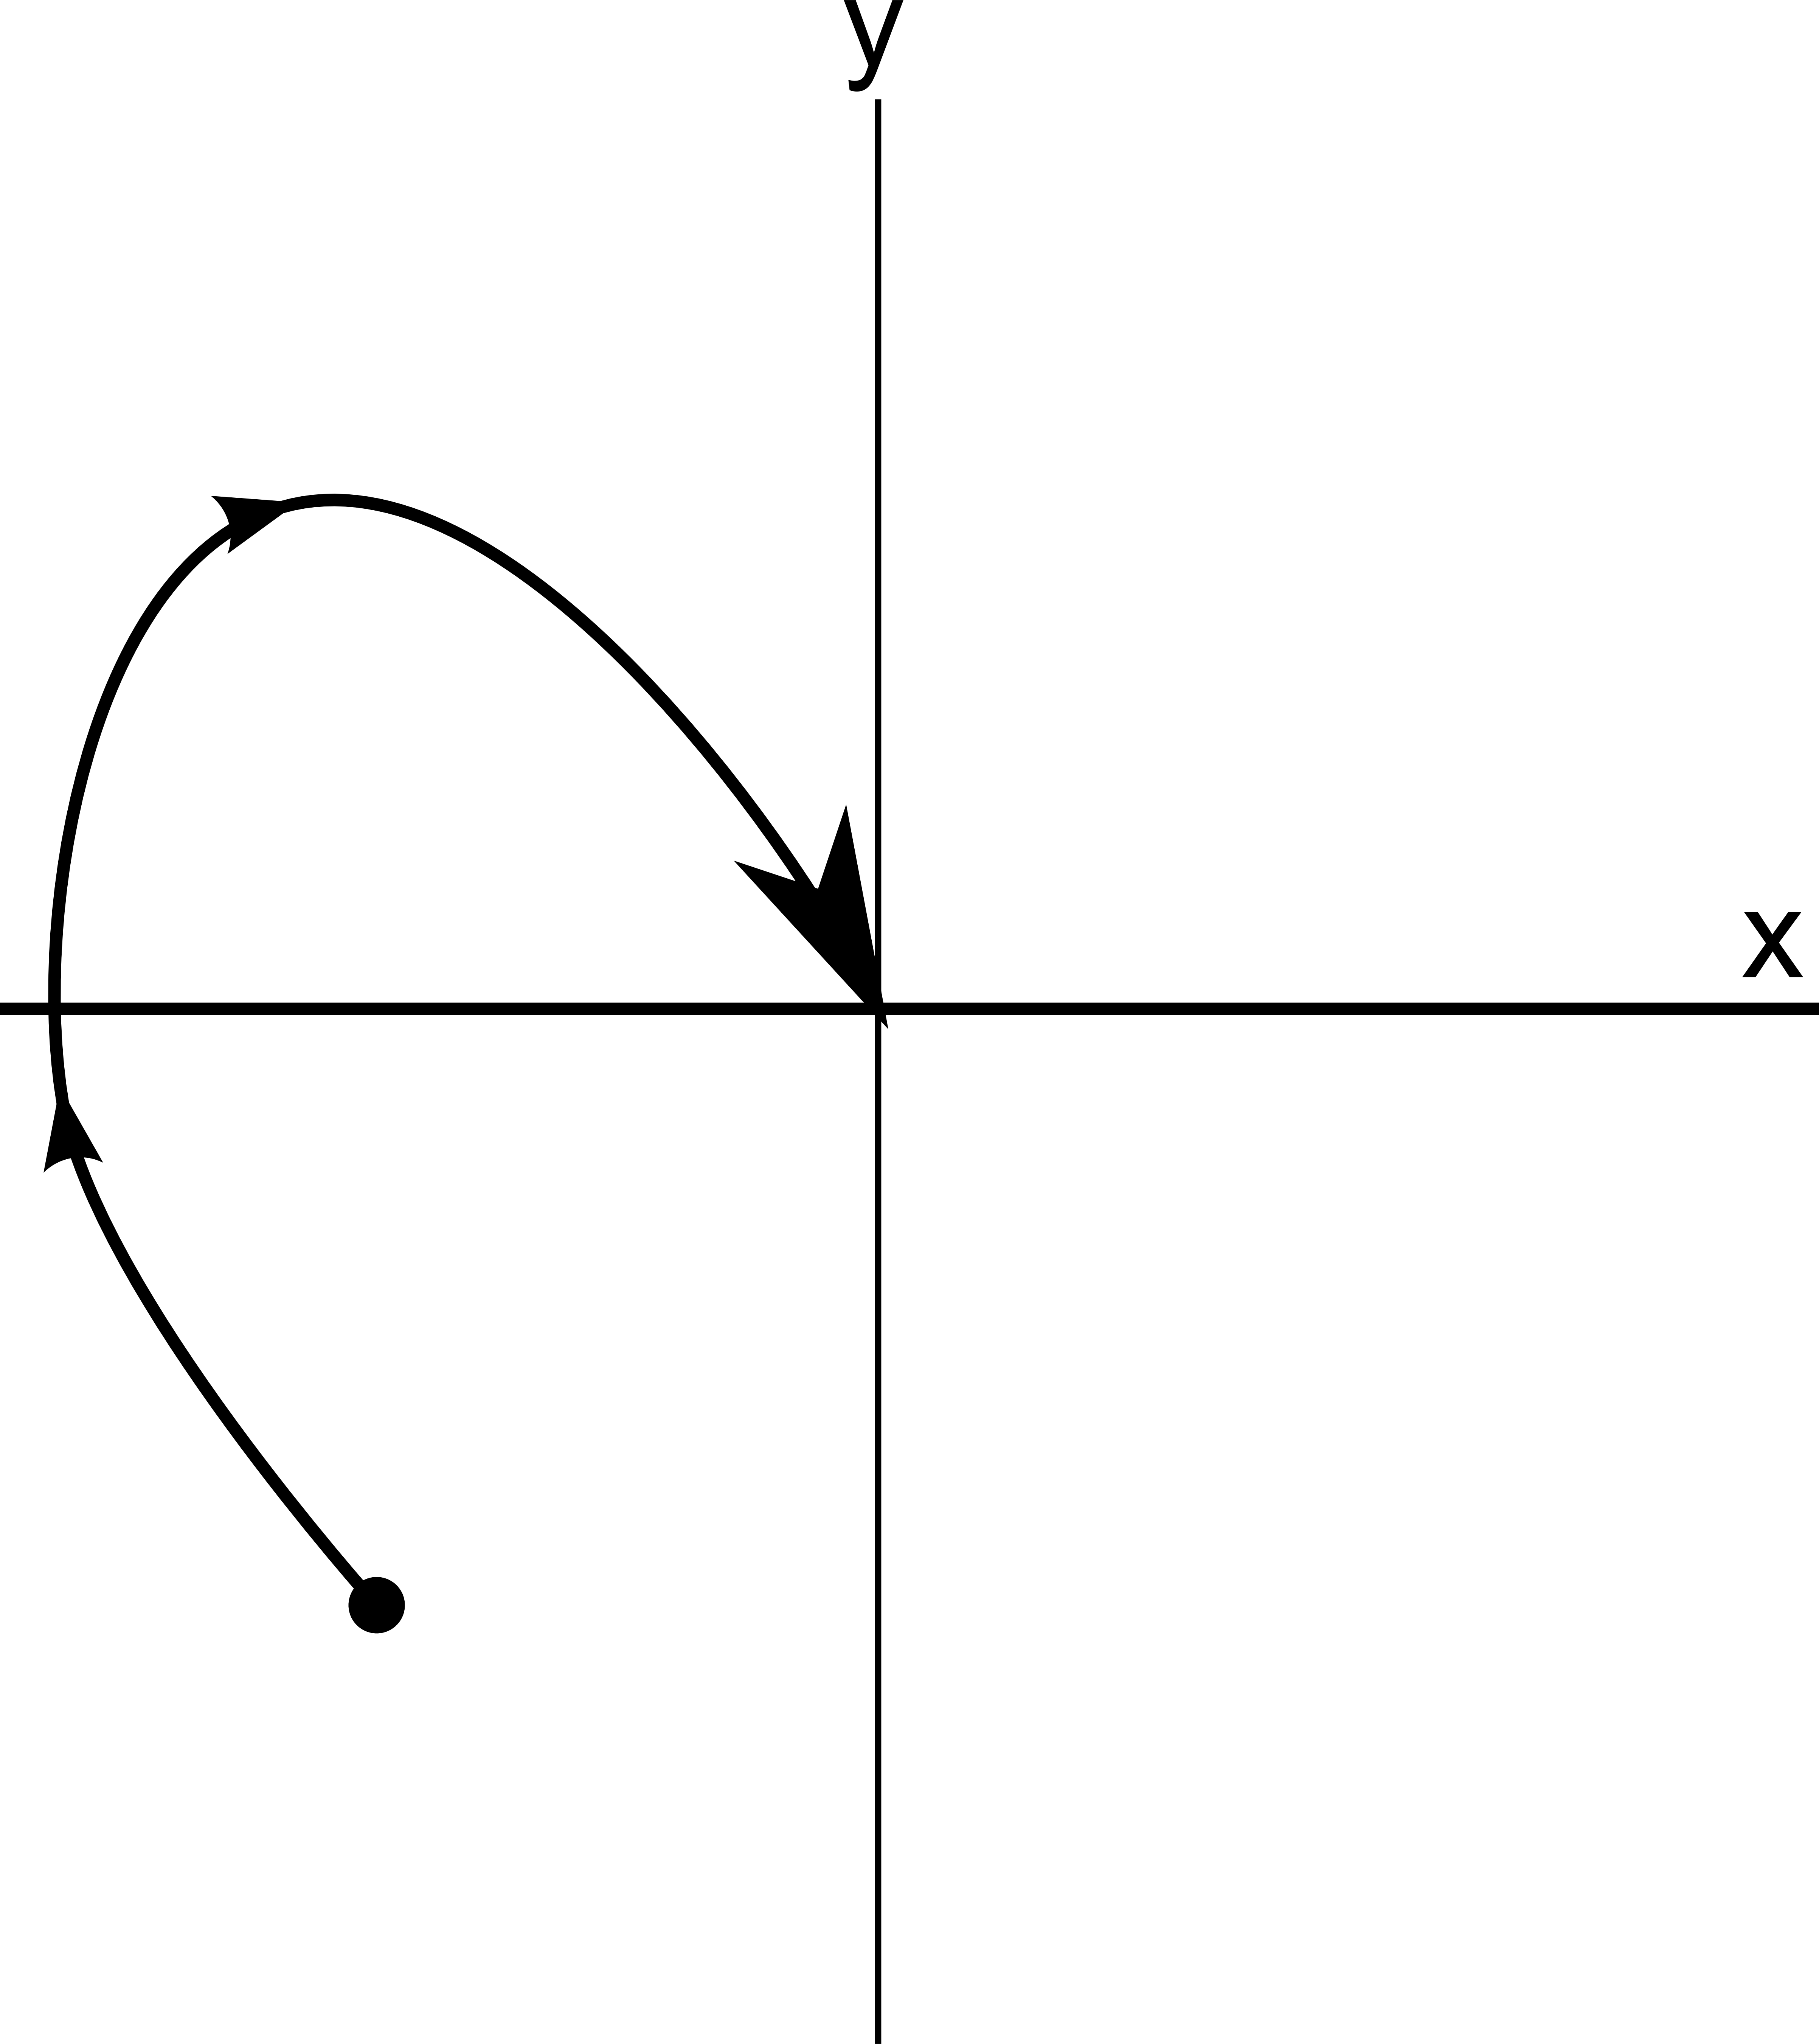
\includegraphics[width=4cm]{img/oneSystemSolution}}
  }

  \only<2->{%
    Phase plane: \\
    \centerline{\includegraphics[width=4cm]{img/phasePlane}}
  }
  

\end{frame}

\subsection{General Framework}

\begin{frame}
  \frametitle{General Solutions}

  \begin{eqnarray*}
    \deriv{~}{t} \vec{x}  & = & A \vec{x} + \vec{f}(t), \\
    \vec{x} & = & \vec{x}_h + \vec{x}_p, \\
    \vec{x}_h & = & \underbrace{C_1 \vec{x}_1(t) + C_2 \vec{x}_2(t) + \cdots + C_n \vec{x}_n(t)}_{n~\mathrm{linearly~independent~vectors}}, \\
    \vec{x}_h & = & \left[ \vec{x_1} \bigg| \vec{x_2} \bigg| \cdots \bigg| \vec{x_n} \right]
    \left[
      \begin{array}{rr}
        C_1 \\ C_2 \\ \vdots \\ C_n
      \end{array}
    \right].
  \end{eqnarray*}

  The vectors, $\vec{x}_i$, are related to the eigenvalues and the eigenvectors.

\end{frame}
\iftoggle{clicker}{%
\begin{frame}
  \frametitle{Clicker Quiz}

   \ifnum\value{clickerQuiz}=1{%
    \vfill

   \begin{eqnarray*}
     \deriv{~}{t} x & = &  4y, \\
     \deriv{~}{t} y & = & -2 x -3y.
   \end{eqnarray*}

   Written in matrix/vector form we get\\[12pt]

   \begin{tabular}{ll}
     A: & $\deriv{~}{t} \vecTwo{x}{y} =  
     \arrayTwo{0}{-2}{4}{-3} \vecTwo{x}{y}.$\\[12pt]
     B: & $\deriv{~}{t} \vecTwo{x}{y} =  
     \arrayTwo{0}{4}{-2}{-3} \vecTwo{x}{y}.$\\[12pt]
   \end{tabular}

   \vfill

 }\fi
  
 \ifnum\value{clickerQuiz}=2{%
   \vfill
   \begin{eqnarray*}
     \deriv{~}{t} x & = &  4y, \\
     \deriv{~}{t} y & = & -2 x -3y.
   \end{eqnarray*}

   Written in matrix/vector form we get\\[12pt]

   \begin{tabular}{ll}
     A: & $\deriv{~}{t} \vecTwo{x}{y} =  
     \arrayTwo{0}{4}{-2}{-3} \vecTwo{x}{y}.$\\[12pt]
     B: & $\deriv{~}{t} \vecTwo{x}{y} =  
     \arrayTwo{0}{-2}{4}{-3} \vecTwo{x}{y}.$\\[12pt]
   \end{tabular}

   \vfill

 }\fi
  
 \ifnum\value{clickerQuiz}=3{%
 \begin{eqnarray*}
    \deriv{~}{t} x & = &  y, \\
    \deriv{~}{t} y & = & -2 x -3y.
  \end{eqnarray*}

   Written in matrix/vector form we get\\[12pt]

   \begin{tabular}{ll}
     A: & $\deriv{~}{t} \vecTwo{x}{y} =  
      \arrayTwo{0}{1}{-2}{-3} \vecTwo{x}{y}.$\\[12pt]
     B: &  $\deriv{~}{t} \vecTwo{x}{y} =  
      \arrayTwo{1}{1}{-2}{-3} \vecTwo{x}{y}.$  \\
    \end{tabular}


        \vfill
 }\fi
\end{frame}
}


\begin{frame}
  \frametitle{Example}
  
  \begin{eqnarray*}
    \deriv{~}{t} x & = &  y, \\
    \deriv{~}{t} y & = & -2 x -3y.
  \end{eqnarray*}

  \uncover<2->
  {
    Written in matrix/vector form we get
    \begin{eqnarray*}
      \deriv{~}{t} \vecTwo{x}{y} & = & 
      \arrayTwo{0}{1}{-2}{-3} \vecTwo{x}{y}.
    \end{eqnarray*}
  }
  
\end{frame}

\begin{frame}
  \frametitle{Find the Eigenvalues and Eigenvectors}

  \begin{eqnarray*}
    A & = & \arrayTwo{0}{1}{-2}{-3}.
  \end{eqnarray*}

  \uncover<2->
  {
    \begin{eqnarray*}
      \begin{array}{rcl@{\hspace{2em}}rcl}
          \lambda_1 & = & -1, & \vec{v}_1 & = & \vecTwo{1}{-1}, \\
          \lambda_2 & = & -2, & \vec{v}_2 & = & \vecTwo{-1}{2}.
        \end{array}
    \end{eqnarray*}
  }

  \uncover<3->
  {
    The solution is
    \begin{eqnarray*}
       \vecTwo{x}{y} & = & C_1 e^{-t} \vecTwo{1}{-1}  + C_2 e^{-2t} \vecTwo{-1}{2}, \\
      x & = & C_1 e^{-t} - C_2 e^{-2t}, \\
      y & = & -C_1 e^{-t} + 2 C_2 e^{-2t}.
    \end{eqnarray*}
  }

\end{frame}


%\subsection{Reducing High Order Systems Using Systems}
\subsection{Reducing High Order Systems}

\begin{frame}
  \frametitle{Tricks of the Trade}

  Suppose that we have
  \begin{eqnarray*}
    x'' + 3x' + 2x & = & 0. \\
    \uncover<2->
    {
      \Rightarrow r^2 + 3r + 2 & = & 0, \\
      (r+2)(r+1) & = & 0, \\
      x & = & C_1 e^{-2t} + C_2 e^{-t}.
    }
  \end{eqnarray*}

\end{frame}


\begin{frame}
  \frametitle{Another Way to Look at It}

  We have
  \begin{eqnarray*}
    x'' + 3x' + 2x & = & 0.
  \end{eqnarray*}

  Let
  \begin{eqnarray*}
    x' & = & y, \\
    \uncover<2->
    {
      x'' & = & y', \\
      y' + 3y + 2x& = & 0, \\
      y' & = & -2x - 3y.
    }
  \end{eqnarray*}

  \uncover<3->
  {
    Written in matrix/vector form we get
    \begin{eqnarray*}
      \deriv{~}{t} \vecTwo{x}{y} & = & \arrayTwo{0}{1}{-2}{-3} \vecTwo{x}{y}.
    \end{eqnarray*}
  }

  \uncover<4->
  {
    \begin{eqnarray*}
      x(t)  & = & C_1 e^{-t} + C_2 e^{-2t}.
    \end{eqnarray*}
  }

\end{frame}


% LocalWords:  Clarkson pausesection hideothersubsections Vicini
